%!TEX root = ../../thirdYearReport.tex
 
\paragraph{Work package 3 progress}

The progress for each task in WP3 is described hereafter.

\subparagraph*{Formulating the control problem (T3.2) (UPMC: 5PM)}

During year 2, a generalized projector has been developed by UPMC and used in \cite{liu-AutRob2015} for hierarchical control. The novelty of hierarchical control algorithms based on the use of this generalized projector is that they can handle not only a single standard lexicographic hierarchy as the HQP and weighting strategies do, but also a complex priority network of hierarchies with both strict and non-strict priorities. The priority between each pair of tasks can be handled separately. Only one swapping phase is needed to move an arbitrary number of tasks to their desired priority levels concurrently.  Moreover, this generalized projector improves the smoothness during hierarchy rearrangements, because it can regulate to what extent a lower-priority task is projected into the null-space of higher-priority tasks (e.g. completely, partially, or not at all). In \cite{liu-AutRob2015}, the generalized projector is implemented in an optimization based dynamic control framework, which is applied to control a KUKA LWR robot in \cite{liu_ICRA2015}. However, the application of this control framework in real-time control of humanoid robots is limited, because its computational cost is sensitive to the number of tasks and the number of DoF of the robot.

The aforementioned generalized projector has also been extended and applied in a quasi-static torque control framework on humanoid robots. Compared with the control framework used in \cite{liu-AutRob2015}, the computational cost of this quasi-static framework is much less sensitive to task numbers or robot complexity. This makes it possible to handle a complex network of task priorities by using the generalized projector, with a computation cost that can be suitable for real-time control of humanoid robots. This work has been experimented on iCub at UPMC and the corresponding results are published in \cite{liu-AutRobSI2015}. Experiments demonstrate that both motion and contact force tasks of different priorities can be handled by this approach. Task priorities can be maintained and switched, and the switching duration can be adjusted to achieve smoother hierarchy rearrangement.

UPMC also started a study in order to evaluate the role, with respect to balance robustness, of a task explicitly aiming at regulating angular momentum to zero in QP-based whole-body controllers. The obtained results are still preliminary but  tend to show, in simulation, that the explicit presence of such a task does not improve the robustness of balance. This work may be further explored during year four.

\subparagraph*{Solving the local control problem (T3.3) (UPMC: 2PM, UB: xPM)}

During year 3, UPMC, UB and IIT worked on solving the whole-body reactive control problem in the case of compliant contact points (see Deliverable~3.2 \cite{deliverable32} and Deliverable~5.3 \cite{deliverable53} for completeness).\\

UPMC finalized the work on the model-free approach retained during year 2. Indeed, when robots evolve in partially known environments, model-based control approaches requires to incrementally, through experience, modify existing models or build new ones (see Deliverable~4.2 \cite{deliverable42} for details on learning of tasks with multiple contacts by imitation and reinforcement learning). While models evolve, the robot still needs to be able to act accordingly, or at least without failure, in this, partially known, environment. Providing an adaptive control approach, not relying on a compliance model, in order to adapt the whole-body motions of humanoid robots to unknown rigidity properties of the environment is thus of interest.

The work contribution of UPMC, following this model-free approach, was published in \cite{liu_IROS2015} and is dedicated to whole-body balancing, and more generally whole-body control, with non-rigid, unilateral, frictional support contacts, for example, standing on a soft ground, or pushing against a compliant support contact with one hand while reaching for an object far away with the other hand (see Fig.\ref{reaching}). The problems of the manipulation of compliant objects and the handling of unexpected disturbance forces are beyond the scope of this work. Moreover, the proposed control approach does not handle anticipatory aspects of balance, but it provides a reactive  mechanism to maintain balance while multiple motion and contact tasks are being performed in a compliant environment.\\
\begin{figure}[!t]
\centering
\vspace{5pt}
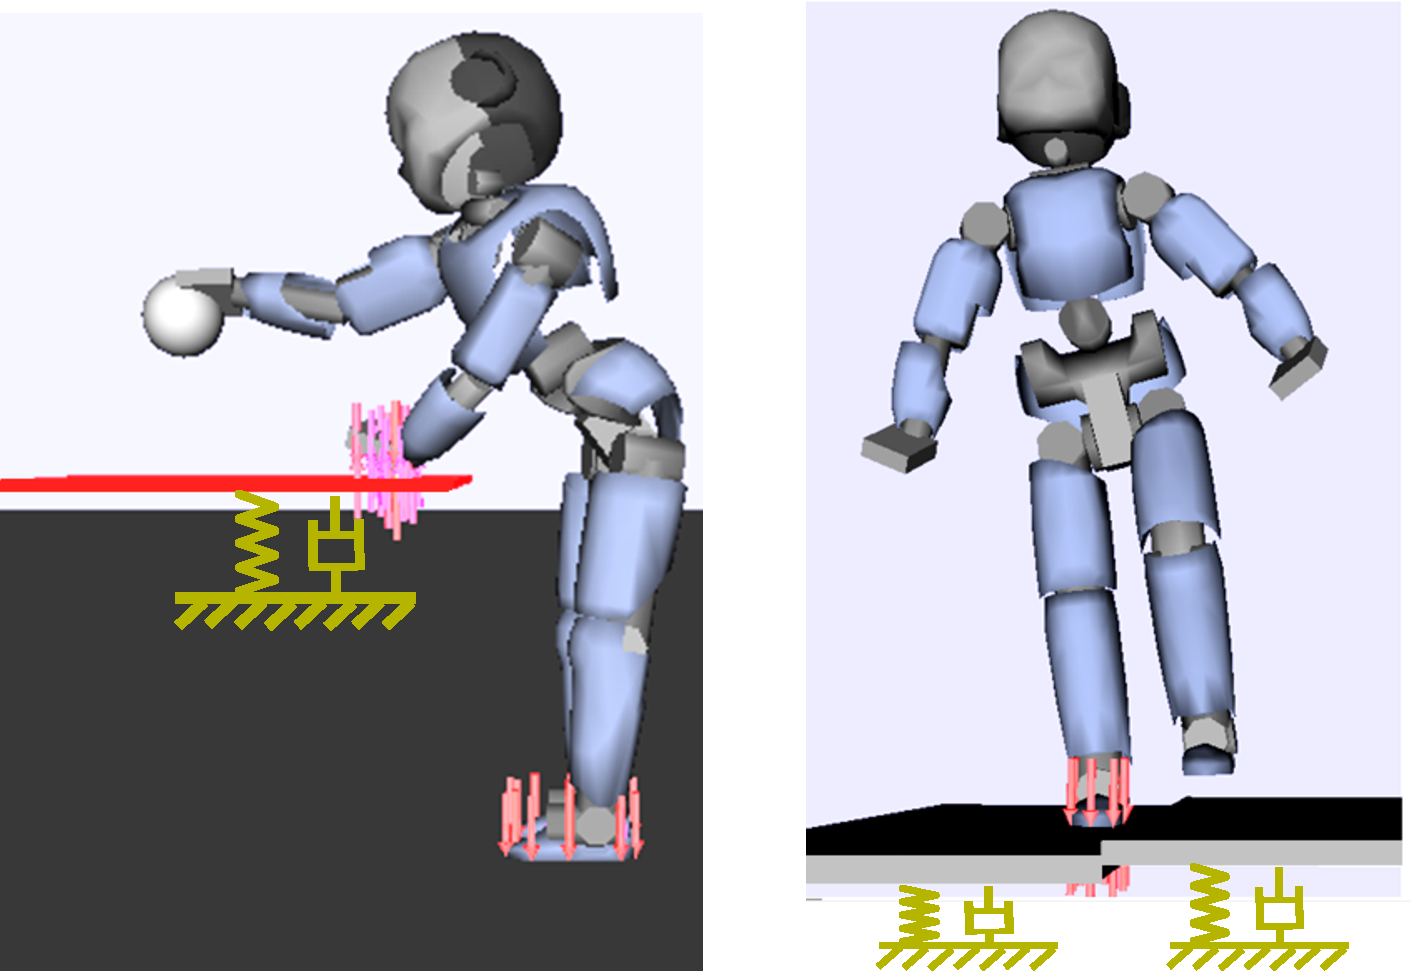
\includegraphics[width=.6\linewidth]{images/scenario.pdf}
\caption{Examples of balancing on non-rigid contacts during whole-body task execution.}
\label{reaching}
\end{figure}

The contribution of this work consists in a reactive controller for whole-body balancing of humanoid robots performing whole-body tasks in unknown compliant environments. As the motions and forces at support contacts are related to whole-body task executions, their reference trajectories are unavailable a priori. Therefore, this approach focuses on the regulation of contact forces in a reactive way. It reacts to the motions of non-rigid contacts in real-time during whole-body movements, with the aim of establishing contact equilibrium quickly.

A frictional non-rigid contact model is proposed both for simulation and for control. The model parameters of the non-rigid environment are unknown to the controller. The force regulation approach does not try to estimate the impedance parameters of the environment, but it regulates contact forces by reacting to environment motions directly. This reactive control approach is embedded in an optimization based multi-task controller of type (1), which has been used to achieve whole-body control of humanoid robots in rigid environments. However, the reactive principle of the approach proposed here is general and can also be applied in many other whole-body controllers to handle non-rigid support contacts.\\ %Examples using this approach are provided, where a humanoid robot performs reaching and stepping actions in a non-rigid environment. Further research directions related to this approach are also presented. Details can be found in the paper hereafter included.

UB followed the model-based approach they had started to derive during year 2. Indeed, when a model of the environment is available or has been incrementally learnt, using this model does not only provide the necessary adaptation to the new conditions but allows to obtain efficient behaviors that could not be obtained otherwise. It thus makes much sense to try to model the compliant environment.\\

When dealing with compliant contacts, modifications are induced in the equation of motion and kinematic constraints expression. The former writes
\begin{equation}
{M}(q) {\dot{\nu}}+{C}({q},{\nu}){\nu} + G(q) = {B} {\tau} + J^\top_{rigid} (q) f_{rigid} + J^\top_{comp} (q) f_{comp}, \label{eq:compliant dyn model}
\end{equation}
while the latter is decomposed in two sub-equations
\begin{subequations}\label{eq:kin constraints}
\begin{eqnarray}
J_{rigid}(q) \dot\nu + \dot{J}_{rigid}(q) \nu & = & 0 \label{eq:kin constraints rigid}\\  
J_{comp}(q) \dot\nu + \dot{J}_{comp}(q) \nu & = & \ddot{p}_{\mathcal{C}_{comp}}\label{eq:kin constraints comp},%(p_{\mathcal{C}_{comp}},R_{\mathcal{C}_{comp}},\dot{p}_{\mathcal{C}_{comp}},\omega_{\mathcal{C}_{comp}},\dot{f}_{comp}) \label{eq:kin constraints rigid},
\end{eqnarray}               
\end{subequations}
where $J^\top_{rigid} (q)$, $f_{rigid}$, $J^\top_{comp} (q)$ and $f_{comp}$ respectively represent the contact Jacobian in the rigid contact directions, the associated rigid contact wrench, the contact Jacobian in the compliant contact directions and the associated compliant contact wrench. Without loss of generality, contacts are here supposed to be either strictly rigid or compliant\footnote{A given contact point can actually be rigid in some direction while compliant in other orthogonal ones.}. $\ddot{p}_{\mathcal{C}_{comp}}$ is the compliant contact points linear and angular acceleration which is assumed to be a function of the state of the contact points and of the derivative of the compliant contact wrench\footnote{As an intuition, consider the example of a mono-dimensional spring-damper system described by the scalar relation $ f = K (x-x_0) + b \dot{x} $, the contact point acceleration can be written $\ddot{x} = \frac{1}{b} ( \dot{f} - K \dot{x})$.} $\ddot{p}_{\mathcal{C}_{comp}} = z\left(p_{\mathcal{C}_{comp}},R_{\mathcal{C}_{comp}},\dot{p}_{\mathcal{C}_{comp}},\omega_{\mathcal{C}_{comp}},\dot{f}_{comp}\right)$.

The Newton-Euler equation for the floating-base system, written at the center of mass of the system, can be written
\begin{equation}
\label{equ:NE equation}
\left( \begin{array}{c}
m (\ddot{x}-g)\\ 
\dot{H}_{\omega}
\end{array}\right) =
\underbrace{\sum_{k=1}^{n_c} \left(\begin{array}{cc}
1_{3} & 0_{3\times 3} \\
S(p_{\mathcal{C}_k} - x) & 1_{3}
\end{array}\right)  f_k}_{X_{\mathcal{C}} f}
\end{equation}
where $m$ is the total mass of the system, $x \in \mathbb{R}^3$ is the position of the center of mass expressed in the inertial frame, $\dot{H}_{\omega}$ is the derivative of the angular momentum, $g$ is the acceleration induced by gravity expressed in the inertial frame, $p_{\mathcal{C}_k}$ is the $k$-contact point and $S(u) \in \mathbb{R}^{3\times 3}$ is the skew-symmetric matrix such that $S(u)v = u \times v$, where $\times$ denotes the cross product operator in $\mathbb{R}^3$.
 
From the modified model, it can be shown that $f$ cannot be considered as an independent intermediate control input any longer as its evolution is subject to the contact points dynamics which is a function of $\dot{f}$. $\dot{f}$ becomes the new independent intermediate control input and it can be concluded that compliant contacts augment the relative degree of the controlled outputs. This means that Equation~(\ref{equ:NE equation}) has to be differentiated in order to relate $\dot{f}$ to the desired center of mass behaviour. The computed contact force derivative can then be fed into Equation~(\ref{eq:kin constraints comp}). Assuming that a good measurement of the compliant contact forces is available and that $z$ can be estimated with high bandwidth and precision through measurement, whole-body dynamics estimation and/or contact model parameters estimation, one can then directly solve the whole-body control problem.\\

Even if not formulated in this way, this is the approach retained by UB in \cite{AzadIROS2015} where a ``practical'' implementation is proposed. The proposed controller regulates both linear momentum and angular momentum about the center of mass of the robot by controlling the contact forces at soft contact surfaces\footnote{rigid contact can be accounted for as well without modifying the proposed method itself and with the advantage of easing the estimation of the state of the floating base}. Assuming that contact forces at the compliant surfaces are known (i.e. via force-torque sensors) at the current instant, desired contact forces at the rigid contacts are calculated in order to provide the required rate of change of the robot's momentum.  However, since compliant contact forces are functions of surface deformations, there is not  any control on them at the current instant. Nonetheless, it is possible to control those forces in the next instant by controlling the acceleration of the contact points.  This can be done by predicting one step ahead in time the compliant contact forces given the currently measured ones and the contact model $z$. To implement the proposed method in practice, stiffness and damping coefficients of the contact model have to be estimated beforehand by using contact model parameter estimation methods such as in \cite{Dallalietal13}, \cite{Diolaitietal05}, \cite{Ericksonetal03}.\\


The contribution of IIT on model-based approaches for dealing with compliant contacts is based on the fact that, in practice, assuming that a good measurement of the compliant contact forces is available and that $z$ can be estimated with high bandwidth and precision through measurement is an illusion. Force measurements are subject to high-frequency noises which in practice limits the bandwidth of the available signal. Moreover, the estimation of the contact model $z$ is complex, and subject to many uncertainties.

There are actually many type of soft terrains that exert forces and torques not only depending on their relative compression, but also on the robot’s joint torques. In these cases, the soft terrain is subject to some rigid constraints that may allow the control of the robot's momentum through the external forces, which thus depend on the joint torques. This is the case of a thin, highly damped carpet, which can be modelled, in the first approximation, as a continuum of vertical springs. Each of these springs is assumed to compress vertically only, and the other degrees of freedom are rigidly constrained, thus creating the aforementioned relation between external forces and joint torques. This brings us back to the case of rigid contacts even though the compliant force component $f_{comp}$ in Equation~(\ref{eq:compliant dyn model}) still needs to be properly compensated for. This particular component cannot be measured separately from the rigid component and a contact model is still needed to estimate it. This approach is the one retained for the demonstration of Year 3 and it is described in details in Deliverable~5.3 \cite{deliverable53}.

 
\subparagraph*{Bootstrapping and validating the control approach in rigid world and compliant cases (T3.4) (UPMC: 1.79PM, TUD: 9.65PM, INRIA: xPM)}
 
In order to ease the deployment of QP-based whole-body controllers, UPMC has put together a set of software libraries named OCRA (Optimization-based Control for Robotics Applications). A short description and links to OCRA are provided in the section dedicated to WP1.

Regarding the use of Model Predictive Control in order to handle the problem of postural balancing under varying contact conditions, the work of N. Perrin \textit{et al.} on two simple and novel approaches to solve for 3D locomotion with multiple non-coplanar contacts has been published in \cite{perrin_ISRR2015}.

During the third year, TUD continued their research in inverse dynamics model learning in presence of dynamic contacts. 
We extended the work from the second year~\cite{Calandra_ICRA15} by integrating the learned models into a controller on the iCub robot.
We evaluated the performance of our mixture-of-contacts approach on real-world tasks such as compensating for contacts with unknown dynamics objects.
An exemplary task is illustrated in Figure~\ref{fig:exp3:icuparis_experiment_bars} when an unexpected obstacle is introduced along the trajectory followed by the arm.
In Figure~\ref{fig:exp3:gating} can be seen the tracking error in presence of an unknown obstacle for multiple control schema. 
It can be noticed how making use of the learned contact models improve the performance compared to simple PD controller or PD plus inverse dynamics.
A paper was published in an international robotics conference~\cite{calandra2015learning}.


\begin{figure*}[h!]
    \centering
    \begin{subfigure}[t]{0.33\textwidth}
        \centering
       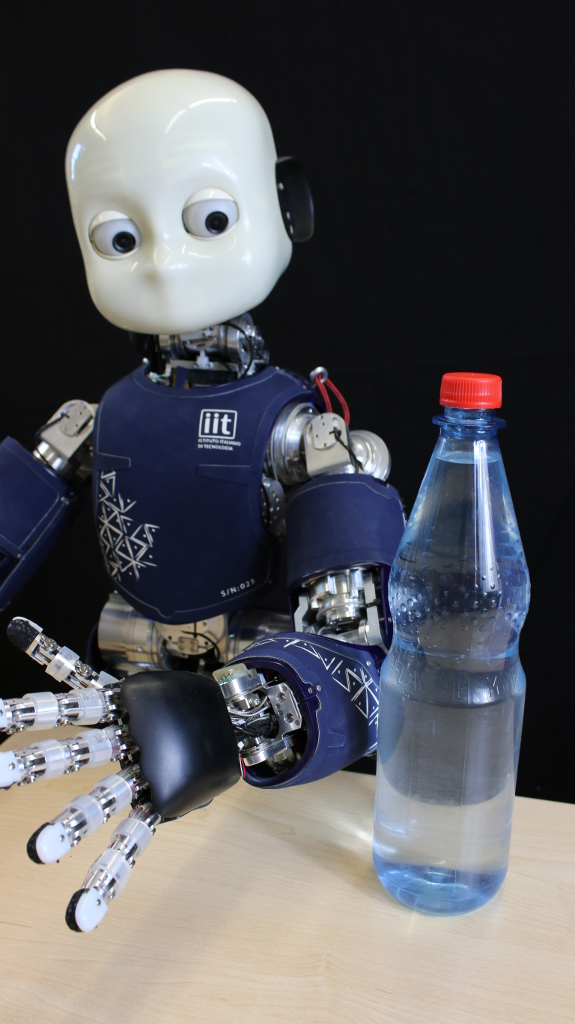
\includegraphics[width =.8\linewidth]{images/taskPush.jpg}
        \caption{The robot during an arm movement encounter an unexpected obstacle. Using the learned contact model the robot compensates for the effects of the obstacle.}
        \label{fig:exp3:icuparis_experiment_bars}
    \end{subfigure}%
    ~ 
    \begin{subfigure}[t]{0.62\textwidth}
        \centering
        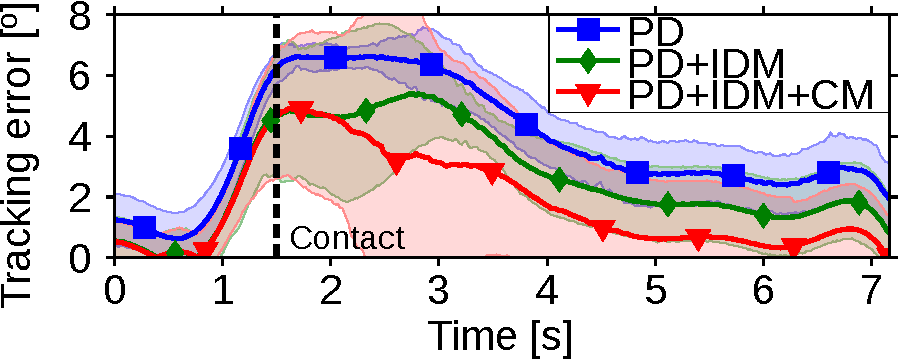
\includegraphics[width=.89\linewidth]{images/trackErrContact3_mod}
        \caption{Tracking error using various control schema. Using the learned contact models improve the tracking performance.}
        \label{fig:exp3:gating}
    \end{subfigure}
    \caption{}
\end{figure*}


In addition, TUD developed a low-cost sensor glove for tele-operating the iCub. The construction and first imitation learning results of object grasping and manipulation were presented in a workshop~\cite{RueckertICRAWS2015}. A description of an improved version of the glove with an in-built IMU and separate sensors for proximal and distal joints was submitted to an international robotics conference. 

INRIA, in collaboration with TUD, has been working on the problem of bootstrapping multi-task controllers with suitable task parametrization. 
In \cite{Modugno2016}, INRIA proposed a simplified multi-task controller based on a linear combination of regularized elementary tasks, where the task weights profiles are parametrized functions that can be automatically optimized offline. The control framework has been applied to the real Jaco Kinova arm and to a simulated KUKA LWR arm.
The description of the learning and optimisation process for the task priorities is postponed in WP4.


\subparagraph*{Extra results in WP2/WP3: UPMC and JSI collaboration (JSI: 2PM, the number of PMs spent by UPMC on this work is counted in WP2)}

UPMC and JSI have been collaborating in order to try to explain curved movement trajectories observed on diagonal reaching movement. This works originates from the study of JSI to elucidate the computational mechanisms of human motor control in situations when humans seek for a supportive hand contact. Within the framework of this study, researchers at JSI performed a series of human experiments where the subjects had to perform diagonal arm reaching to targets of different sizes. Human reaching studies often focus on reaching forward in the sagittal plane, which commonly results in straighttrajectories \cite{ThoroughmanNature2000}. However, slightly curved reaching trajectories were also observed \cite{IzawaJNeuro2008}, \cite{UnoBioCyber1989}. Reported curvatures were very small, possibly due to small movement amplitudes. JSI investigated whether large amplitude movements outside of the sagittal plane show larger deviations from straight line trajectories.

Ten healthy, seated males ($20 \pm 2.7$ years) reached with their dominant right arm to a virtual target using a haptic manipulator, which constrained the motion to the horizontal plane at shoulder height and emulated a uniformly viscous media. The virtual target (width $5mm$) was centered to the subject’s shoulder and positioned at a virtual wall at $95\%$ of arm length. Reaching movements started from random starting points (SPs) evenly distributed within $\pm 45^{\circ}$ around the target at distances of $15\%$ (three SPs), $37.5\%$ (five SPs), and $60\%$ (seven SPs) of arm length. Subjects were to position the cursor at a given SP and move anytime following a ready signal. Movement duration, from self-initiated reach onset to reaching the virtual wall, was calculated for each reach and subjects were instructed to hit the target as many times as possible in a total movement time of 100 s. Each target hit was rewarded by $0.025$ euros. Accumulated reward, remaining time, target, SP, and visual feedback of the hand cursor were shown in real time. Overall reach accuracy was comparable across all SPs.
Kinematic data were analysed for reaches starting from $+45^{\circ}$ (rightward diagonal reach), $-45^{\circ}$ (leftward diagonal) and $0^{\circ}$ (straight) at the three SPs distances. Trajectory length and movement duration were calculated for 307 accurate target hits and averaged over subjects and SPs. Following a paired t-test $+45^{\circ}$ and $-45^{\circ}$ SP data were collapsed. Statistics were conducted at $\alpha = 0.05$.

Trajectories differed significantly from the Euclidean distances between the SP and the target for all $45^{\circ}$ SPs ($0.9~–~1.3 cm$) longer, paired t-test all $p<0.02$) and for $0^{\circ}$ SP at the shortest distance ($2mm$, paired t-test $p = 0.02$). Angle influenced both trajectory prolongation and duration, but distance between the target and the SP affected only movement duration ($p < 0.02$ for all, repeated measures ANOVA).

Subjects reached the target with equal success from all SPs, but their movement trajectories were curved when reaching at $45^{\circ}$, unlike mostly straight movements at $0^{\circ}$. Such behaviour might reflect task generalization to reaching forward in the sagittal plane\cite{GallivanNatureCom2015}, possibly due to complexities caused by different SPs. Computational modelling of this behaviour, taking into account the underlying muscle activity, is performed by UPMC.


To this end, UPMC has proposed a computational model of reaching movements designed to explain the phenomena studied experimentally by JSI. The model unifies a cost-benefit trade-off \cite{rigoux12_plos} and a speed-accuracy trade-off \cite{fitts54_JEP} to explain movement properties related to time. Precision constraints are incorporated through the derivation of an optimization criterion that considers probabilistic reaching of a rewarding target that may be missed if the motion is too fast.

The model has been coded in python. The movement controller is implemented as an artificial neural network to which supervised learning (aka regression) is applied to obtain a initial good enough behaviour. Once this controller is initialized, an optimization process is applied to 4 instances of the weights of the artificial neural network to obtain 4 different controllers whose behaviour is optimized to 4 different target sizes. We then check the properties of the obtained controllers with respect to what is expected from the experimental movements recorded at JSI. The results are depicted in \figurename~\ref{fig:trajs} to~\ref{fig:hitdisp}.

\begin{figure*}[t!]
 \centering
  \begin{subfigure}[t]{0.45\textwidth}
    \centering
    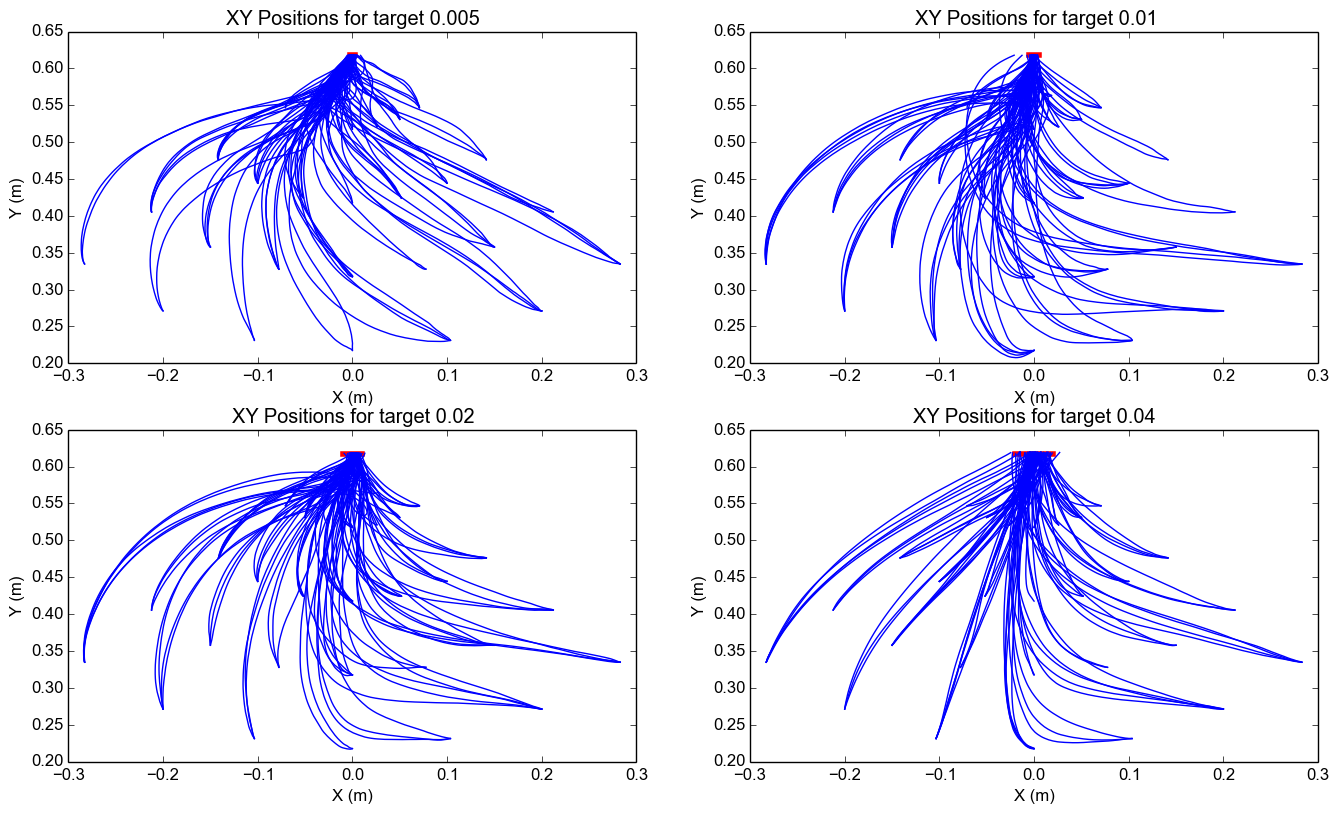
\includegraphics[width=0.9\linewidth]{images/trajs.png}
    \caption{Reaching trajectories obtained with the four optimized controllers.\label{fig:trajs}}
  \end{subfigure}%
  ~ 
  \begin{subfigure}[t]{0.45\textwidth}
    \centering
    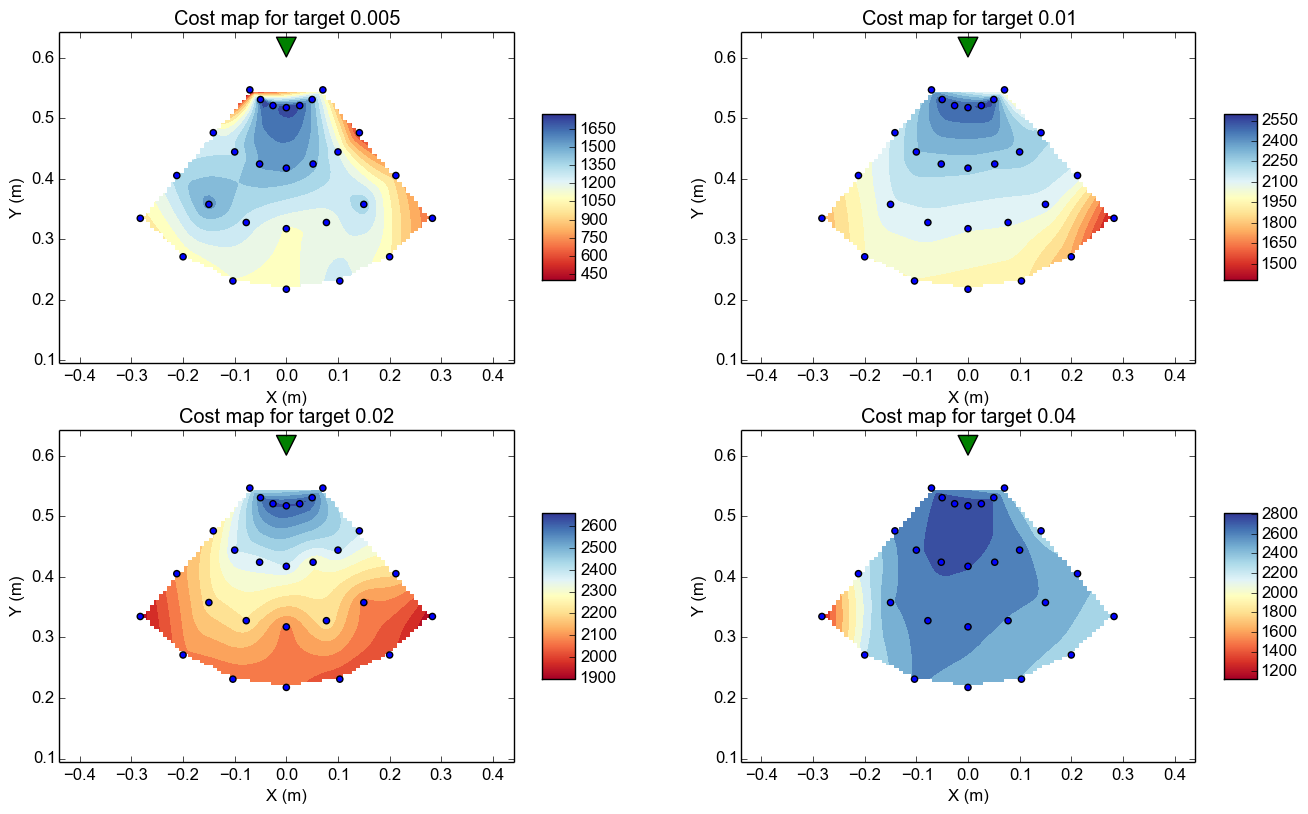
\includegraphics[width=0.9\linewidth]{images/costmap.png}
    \caption{Cost of movement from any starting point to reach the 4 different targets.\label{fig:costmap}}
  \end{subfigure}%
  \linebreak
	\centering
  \begin{subfigure}[t]{0.45\textwidth}
    \centering
    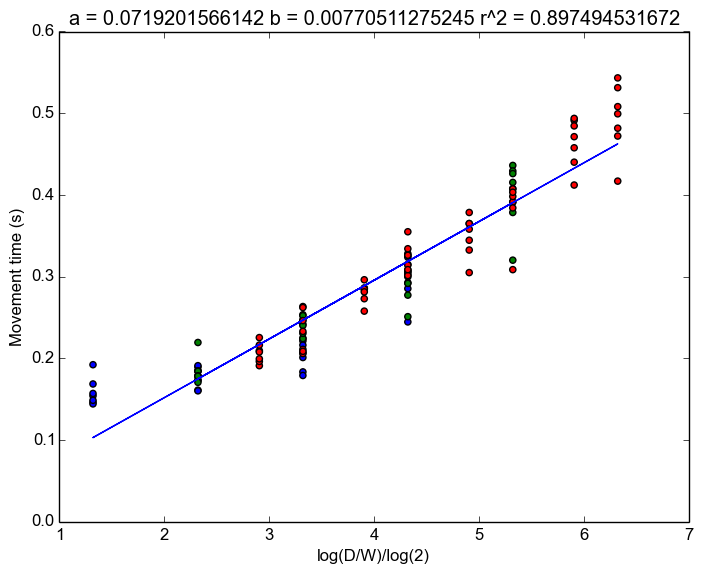
\includegraphics[width=0.8\linewidth]{images/fitts.png}
    \caption{Reproduction of Fitts' law obtained from the data above.\label{fig:fitts}}
  \end{subfigure}%
  ~ 
  \begin{subfigure}[t]{0.45\textwidth}
    \centering
    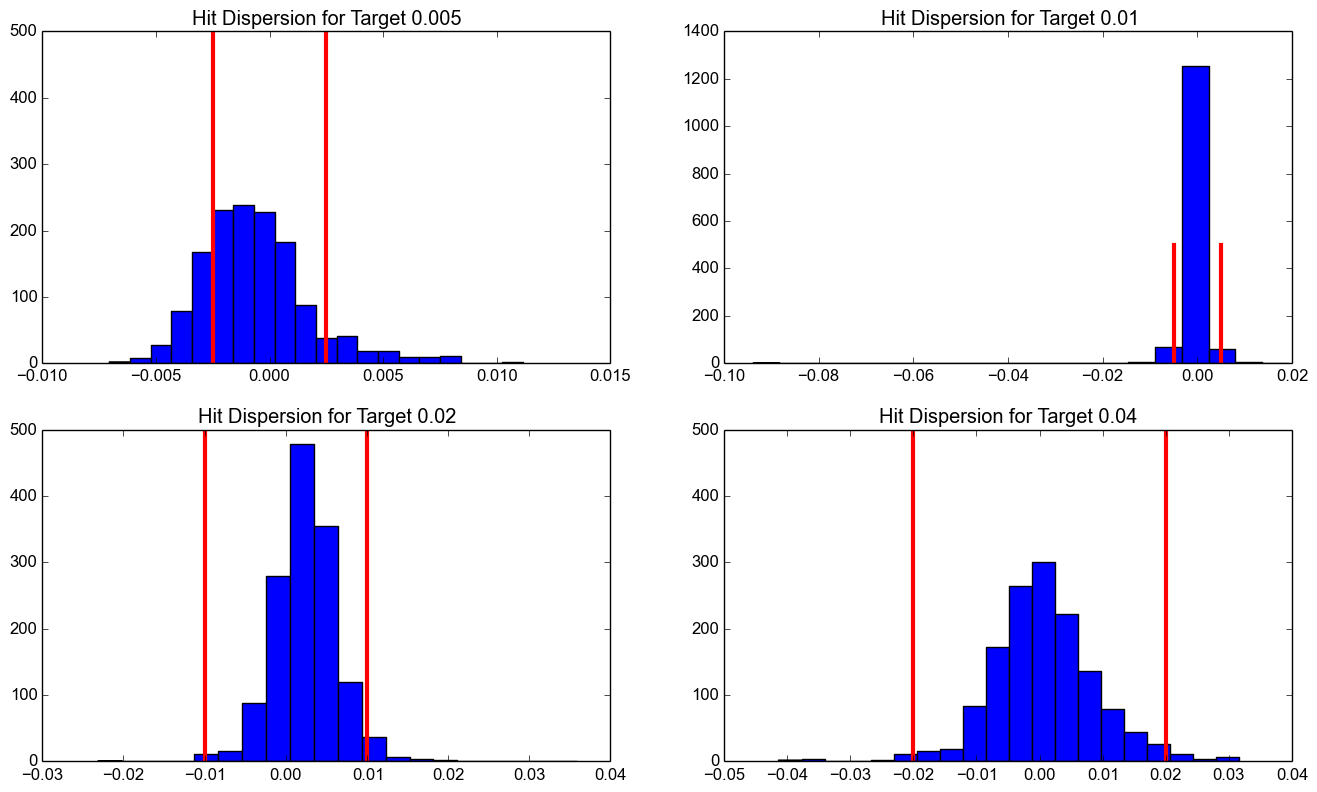
\includegraphics[width=0.9\linewidth]{images/hitdisp.png}
    \caption{Hit dispersion obtained with the four optimized controllers.\label{fig:hitdisp}}
  \end{subfigure}%
  \caption{}
\end{figure*}

As one can see, the model consistently obtains Fitts' law (\figurename~\ref{fig:fitts}), with a very good $r^2$ factor of $0.90$ (to be compared to the $0.92$ obtained by JSI on human movements). The maps showing the cost of movement as a function of the starting point (\figurename~\ref{fig:costmap}) are also consistent with the ones of JSI, as is also the case with the hit point dispersion depending on the size of the target (\figurename~\ref{fig:hitdisp}). Globally, the modelled arm controller is able to slow down to improve accuracy of reaching when the targets are smaller, which was the main expected outcome of the model. The velocity profiles of the corresponding movements (not shown) are also satisfactory.
However, the obtained reaching trajectories (\figurename~\ref{fig:trajs}) are more curved than those recorded at JSI. We are currently investigating the potential impact of the optimization process on this phenomenon and envisioning using new deep reinforcement learning tools \cite{lillicrap2015continuous} instead of stochastic optimization \cite{hansen2003reducing} to accelerate the optimization process.
 


 
